% !TEX root = ../Yan Hao--Dissertation.tex

\chapter{Questions on the Central Level}
% Fiscal federalism is a form of fiscal decentralization that is widely recognized as a more efficient way to provide public goods and services, particularly in large and complex countries with multiple levels of administrative institutions. Hayek \cite{hayek2009use} argued that local governments are better positioned to understand local needs and preferences, and therefore to provide appropriate public goods and services. Stigler \cite{stigler1998tenable} built on Hayek's insights and argued for the necessity of protecting the funding ability of subnational governments. Tiebout \cite{tiebout1956pure} developed a theoretical framework to show that voting with one's feet can ensure that public goods supply matches local needs. He also demonstrated that competition among local governments can lead to improved administrative efficiency. Tiebout's theory seems get supported by the actual data showed in Table \ref*{Table 2.1}, which potentially reflects the difference of tax burden preference of different states. These foundational insights form the basis for much of the research on the advantages of fiscal federalism. For the following part, I'll focus on the evaluation of decentralized fiscal structure which is fiscal federalism.


% % Table generated by Excel2LaTeX from sheet 'Sheet1'
% \begin{table}[H]
%     \centering
%     \caption{Effective Tax Revenue in America}
%     \begin{tabular}{p{9.43em}lll}
%         \toprule
%         State                & \multicolumn{1}{p{8.145em}}{State and Local Taxes (\$ billions)} & \multicolumn{1}{p{7.43em}}{Personal Income (\$ billions)} & \multicolumn{1}{p{9.93em}}{Effective Tax Rate} \\
%         \midrule
%         New York             & \multicolumn{1}{c}{177.8}                                        & \multicolumn{1}{c}{1,281.10}                              & \multicolumn{1}{c}{13.90\%}                    \\
%         District of Columbia & \multicolumn{1}{c}{7.5}                                          & \multicolumn{1}{c}{55.5}                                  & \multicolumn{1}{c}{13.40\%}                    \\
%         North Dakota         & \multicolumn{1}{c}{5}                                            & \multicolumn{1}{c}{39.5}                                  & \multicolumn{1}{c}{12.70\%}                    \\
%         Hawaii               & \multicolumn{1}{c}{9.5}                                          & \multicolumn{1}{c}{75.4}                                  & \multicolumn{1}{c}{12.60\%}                    \\
%         Vermont              & \multicolumn{1}{c}{3.8}                                          & \multicolumn{1}{c}{32.6}                                  & \multicolumn{1}{c}{11.70\%}                    \\
%         \midrule
%         United States Total  & \multicolumn{1}{c}{1,652.80}                                     & \multicolumn{1}{c}{16,820.30}                             & \multicolumn{1}{c}{9.80\%}                     \\
%         \midrule
%         Alabama              & \multicolumn{1}{c}{16.4}                                         & \multicolumn{1}{c}{198.9}                                 & \multicolumn{1}{c}{8.30\%}                     \\
%         Oklahoma             & \multicolumn{1}{c}{13.9}                                         & \multicolumn{1}{c}{174.4}                                 & \multicolumn{1}{c}{8.00\%}                     \\
%         \midrule
%         \multicolumn{4}{p{34.935em}}{\textit{Source:U.S. Census Bureau Dataset}}                                                                                                                             \\
%     \end{tabular}%
%     \label{Table 2.1}%
% \end{table}%


% \section{How to Evaluate the Fiscal Federalism System}
% Even within the topic of fiscal federalism, the fiscal federalism structures in different countries have different content and features, needless to say, they show different impact in public goods and services supplying. Like I mentioned in Chapter 1, it's hard and nearly impossible to find a perfect stick yard criterion to compare fiscal federalism in different countries. I'll try to explain and get a comprehensive way to evaluate fiscal federalism. Literature about fiscal federalism can be roughly divided into two groups. First-generation theory of fiscal federalism concentrate on the fiscal structure itself, focusing on the efficiency of federalism in collecting revenue and offering responsibilities, and whether the revenue-responsibility combination perform well in public goods supply. Coming to second-generation theory of fiscal federalism, scholars get interested in the effect of fiscal federalism on other area such as the effect on economic development.

% \subsection{First-Generation Theory of Fiscal Federalism}

% Evaluating the efficiency of fiscal structures is a common approach to assessing their reasonableness. Pareto efficiency, which requires that resources be allocated in a manner that cannot make anyone better off without making someone else worse off, is widely accepted as a standard for evaluation \cite{pareto2014manual}. Scholars have identified three economic factors useful in evaluating fiscal structures: externalities, information complexity, and incentive compatibility. Oates \cite{oates1972fiscal} proposed that governments and residents of a jurisdiction should bear the costs of negative externalities and receive payment for positive externalities. Olson \cite{olson1993dictatorship} argued that the "free rider" problem could be resolved by making jurisdictions and beneficiary areas identical, achieving an equilibrium in which marginal costs equal marginal benefits. One example of an efficiency consideration in the United States' fiscal federalism structure is the revenue structure for individual taxes, as shown in Table \ref*{Table 2.2}. To minimize behavioral distortions and improve efficiency, individual income taxes, which are easy to move across jurisdictions, are mainly collected by federal and state governments, allowing individuals to be indifferent about where they live and pay taxes.

% % Table generated by Excel2LaTeX from sheet 'Sheet1'
% \begin{table}[htbp]
%     \centering
%     \caption{. Percentage Composition of Tax Revenue by Government Level}
%     \begin{tabular}{lccc}
%         \toprule
%         \multicolumn{1}{c}{Type} & Federal & State   & Local   \\
%         \midrule
%         Individual income        & 51.80\% & 37.20\% & 4.70\%  \\
%         Corporate income         & 6.90\%  & 4.70\%  & 1.10\%  \\
%         Other taxes              & 41.20\% & 58.10\% & 94.20\% \\
%         \bottomrule
%     \end{tabular}%
%     \label{Table 2.2}%
% \end{table}%


% Besides, information complexity is an important consideration in evaluating fiscal federalism structure. Basing their work on the earlier contributions of Hayek and Tiebout, Bseley et al \cite{2003Centralized} developed a political economy model to simulate the decision-making process in a democratic country. They emphasized the advantage of local government in public goods supplying and introduced insensitivity of central government into their model. Information communication is also important, with local governments having better knowledge of local residents' needs and their behavior being better perceived by local residents. Decentralized fiscal federalism structures put local governments under supervision, as noted by Dethier \cite{martinez2003fiscal} and based on Tiebout's voting on feet framework. Baicker \cite{baicker2005spillover} introduced a horizontal competition structure with multiple local governments and states that enables local residents to evaluate local governments' efficiency in public goods supply under a yardstick competition framework. This information transparency can push local governments to improve their performance.

% Finally, a well-designed fiscal structure should satisfy the criterion of incentive compatibility. Incentive compatibility is a game theory concept introduced by Leonid Hurwicz \cite{hurwicz1973design} that requires a mechanism to be designed such that each participant can achieve the best outcome for themselves by acting truthfully. In public administration and public economics, incentive compatibility has become an important criterion for evaluating the quality of fiscal federalism. Proper fiscal federalism settings can motivate local governments to efficiently provide public goods. For example, Eckstein \cite{eckstein1958water} argues that the proper combination of funding resources and responsibilities can motivate organizations, including local governments, to work hard and provide public goods efficiently, since working hard with efficiency in public goods supplying is an weakly dominate strategy and could attract more residents and increase more public funding resource. Under the impact of incentive compatibility theory, scholars generally assume that local governments aim to maximize local fiscal revenue in fiscal federalism administration process. (Baretti, Bucovetsky,Dahlby,Jha) \cite{baretti2002tax,bucovetsky2006efficiency,dahlby2011marginal,jha2000tax}.

% The first-generation theory of fiscal federalism focuses on the positive impact of decentralized structures on public goods provision. The main research objective is to assess the effectiveness of fiscal federalism in enhancing public goods efficiency. This period is characterized by theoretical studies.

% \subsection{Second-Generation Theory of Fiscal Federalism}

% The second-generation theories of fiscal federalism expand beyond the efficiency of public goods provision and explore its impact on other social areas, such as economic development \cite{cai2005does,barro1991economic} and local government behavior \cite{jin2005regional}. Once connect the fiscal federalism with other social areas, scholars in this generation highlight that fiscal federalism may not always function effectively, particularly in developing countries \cite{keen1997fiscal,treisman2002decentralization,bardhan2002decentralization,bucovetsky2005public}, while acknowledging the fundamental role of fiscal federalism in public goods provision. The literature can be categorized into three themes: the relationship with economic development, political intentions, and its effect on local government fiscal behavior.

% The relationship between fiscal federalism and economic development is inspired by Charls Tiebout's theory \cite{tiebout1956pure}, which has been supported by ample econometric evidence. However, Tiebout's theory is based on assumptions that are hard to achieve in developing countries, where local governments may not have the ability to supply public goods with proper efficiency. Second-generation theory literature aims to explore the limitations of Tiebout's assumptions and investigate the implications for economic development. The role of production factors such as labor and capital in fiscal federalism has been studied extensively. Econometric evidence suggesting that even within developed countries like the European Union, residents do not move freely between jurisdictions \cite{oates2004essay}. Faguet's survey found that even for those who do move, public goods performance is not their primary concern \cite{faguet2004does}. Except for the population movement, capital is also a interesting factor in fiscal federalism literature. Mckinnon \cite{mckinnon1993order} attribute the economic boost in southern United States to the low factor cost including capital, labor and land. He then did a follow up research claims that the compensation and equalization effect of transfer payment in fiscal federalism system may block the flow of production factors. Cai and Treisman \cite{cai2005does} proved that with initial difference in resource endowment, the decentralized feature of fiscal federalism may lead to local governments' sturdiness in economic development since the moving of capital seems surely lead to development imbalance, the imbalance between different jurisdictions will destroy the enthusiasm of local governments. Treisman \cite{treisman2002decentralization} further emphasizes that such governments with lower resource endowments tend to prioritize poverty reduction over economic development efficiency.

% Scholars of second-generation theory have noted the impact of fiscal federalism on local government behavior, including the influence of intergovernmental transfers on local tax collection efforts \cite{mogues2012external}, spending structures \cite{hines1995anomalies}, and debt \cite{qian1998federalism}. These effects will be further analyzed in Chapter 3 under asymmetric conditions.

% In addition to economic considerations, political intentions also play a significant role in explaining fiscal federalism design. While economic and efficiency theories are commonly used to explain fiscal federalism, political factors can be a fair supplement in explaining fiscal policy and behavior. In Canada, fiscal federalism is an important tool for equalizing resources across different jurisdictions and serves as a glue for political federalism. Similar econometric evidence is found in Australia as well \cite{oates2005toward}. However, the transfer payment mechanism from high fiscal revenue areas to low revenue areas in Italy has exacerbated conflicts between different jurisdictions, leading to a different look for fiscal federalism in Italy.

% Except for the relationship between revenue and responsibilities within individual jurisdictions, the interaction between governments is a compelling topic for researchers in the field of fiscal federalism. This interaction can be broadly divided into two categories: horizontal interaction, which refers to the interaction among governments at the same level, and vertical interaction, which refers to the interaction between central and subnational governments. In this paper, the focus will be on the vertical interaction between central and subnational governments.


% \begin{figure}[H]
%     \centering
%     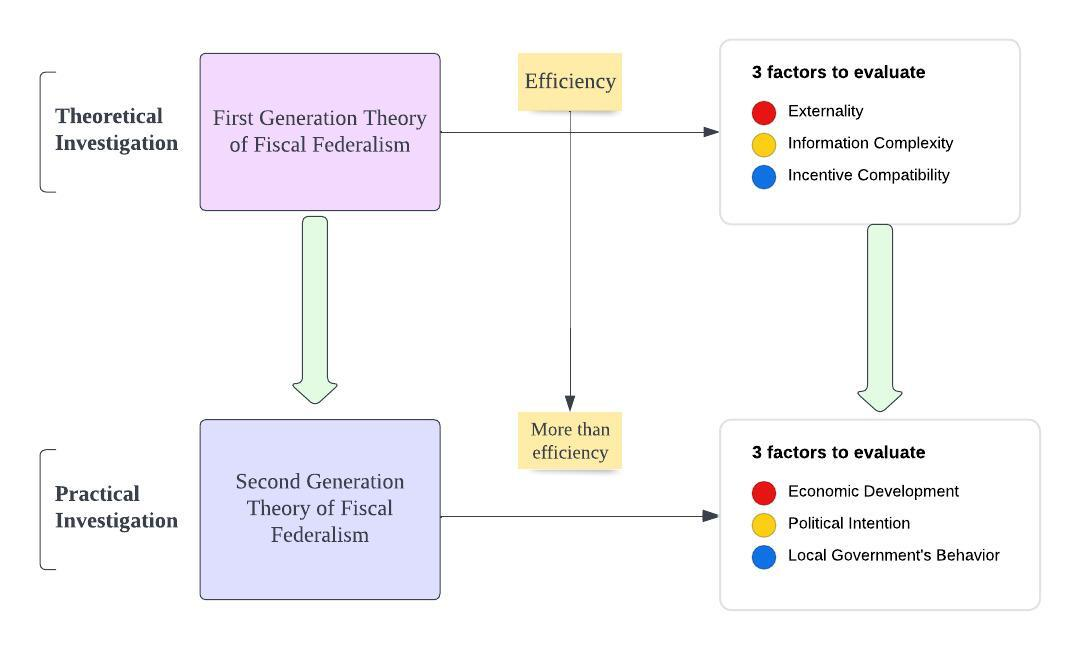
\includegraphics[scale=1]{Chapter-2/Figures/how to evaluate the fiscal federalism.jpeg}
%     \caption[How to evaluate the fiscal federalism]{How to evaluate the fiscal federalism
%         \texttt{} }
%     \label{Figure 2.1}
% \end{figure}

% In summary, as depicted in Figure \ref*{Figure 2.1}, the original research on fiscal federalism constructed a theoretical framework for efficiently providing public goods. In developed countries, particularly in America, scholars have discovered empirical evidence supporting the advantages of this decentralized fiscal structure. However, in developing countries, fiscal federalism has not worked as effectively, leading to the emergence of second-generation theory. This newer approach focuses on the other side of the coin.


\section{National Government's Choice}
As mentioned in Chapter 1, broadly there are three choices available for national government when dealing with the provision of sublevel jurisdictions' public goods, which are no provision, joint provision and intergovernmental transfer. Based on Volden's \cite{volden2007intergovernmental} dynamic game setting, I expand his setting in three aspects to better investigate governments' behavior. Firstly, I differentiate the intergovernmental transfer into transfer with bare restriction--general transfer and transfer with restriction attached--categorical transfer. Secondly, I assume different kinds of players on subnational level in terms of the resource endowment. Besides, I modified the utility preference for the players in this game compared to Volden's setting. I'm listing my game setting in detail specifically in following sections.

\section{A Dynamic Game Analysis with Complete Information}
The Figure 2.1 demonstrates the extensive form of central and subnational interaction, which is developed based on Volden's game theory model \cite{volden2007intergovernmental}.But this paper presents a modified version of the game. Departing from Volden's model, I consider two types of players differentiating in the tax base (or resource endowment) instead of assuming identical subnational governments. Moreover, the paper defines different types of grants and specifies varying restrictions attached to grants. Additionally, the game in this paper incorporates a different form about the utility of subnational governments by considering the free rider risk. The game model in this paper can be described in terms of three aspects: player set, behavior set, and utility set.The nuance of the difference between the modal in this paper and Volden's model will be explained in detail in following sections. Besides, the game is set as a dynamic game with complete information, which means the utility for all players in this game is a common knowledge for all players. In summary, the modified game in this paper offers a more nuanced understanding of the interactions between central and subnational governments.

\begin{itemize}
\item \textbf{Player Set}\\
Three players take actions in this intergovernmental transfer game: the central government $N$, state governments with higher resource endowment $S_h$, and state governments with lower resource endowment $S_l$. The assumption of identical subnational governments in Volden's paper is relaxed. Since governments with differing resource endowments may have varying fiscal preferences, leading to differing reactions to intergovernmental fiscal policy. The player set can be listed as $P = \{ N, S_h, S_l\}$. For convenience, I defined $i\in \{l,h\}$. \label{player} The difference between $S_h$ and $S_l$ is that the states with higher resource endowment is more productive, possess higher tax bases (GDP), thus I have $F_h>F_l$\label{GDP}.

\item \textbf{Action Set}\\
For central or national government, one available choice for national government is to stay out of the subnational jurisdictions' public goods provision. I call this subgame as no provision game. Otherwise, once the national government decide to join the provision, next question is to decide how to join, the available choices are joint provision game, general transfer game or categorical transfer game. Joint provision game is to provide the goods directly. In this case, citizens in a specific state enjoy the public goods offered by both national and subnational governments combined.In joint provision game, the national government is the direct provider of the goods and decide the amount of public goods provided to $S_i$, which are $G_{Ni}$.

Another subgame is to offer intergovernmental transfer. In Volden's setting, national government can offer grants only through general transfer, which is a lump-sum subsidy. I assume there are two kinds of intergovernmental transfer. Transfer to lower level governments are either general transfer $GT$ or categorical transfer $CT$ which is more restricted during administrative process and subnational governments cannot use the grants freely as they want to. \label{transfer} Volden didn't distinguish different kinds of grants in his dynamic game setting. However the restriction may play a role in affecting both national and subnational governments' behavior, thus I differentiate the intergovernmental transfer in terms of the restriction level following Table \ref{Table 1.3}.

The main goal of the national government to join the general transfer subgame is to narrow the utility gap of $S_i$ and equalize the original resource endowment difference. The effect of general transfer has been wildly mentioned in fiscal federalism literatures \cite{buettner2006incentive,lv2018transfer}. I adopted Buettner's design about the amount of general transfer, in which general transfer amount $T$ received by government $i$ can be captured as:
$$T_i = T_0 - \sigma F_i $$ \label{generaltransfer}
where $\sigma$ captures the central government's intention to equalize the resource in different jurisdictions. A higher $\sigma$ means national government prefer to equalize the resource. For example, compared to US government, OECD central government prefer to set a higher $\sigma$. $T_0$ is the benchmark grants amounts when $S_i$ got zero $F_i$. $F_i$ is the total production output which is also the tax base of $S_i$.

Compare with the general transfer, the equity is not a main concern in categorical transfer game. The role for categorical grants is to affect the policy direction in subnational jurisdictions. By encouraging the spending in specific area, central government could achieve the policy output in a national-favored direction. The categorical transfer are typically matching transfer, which means national government pay for specific percentage of the expenditure in specific area and subnational governments pay for the rest. I assume there are two kinds of public goods on subnational level which are productive goods $P$ like roads, railways, and other kinds of infrastructure. Another kind of public good is welfare public goods $W$ like social welfare, salaries for public servants.

For categorical transfer game, I assume matching ratio for productive grants is $m$ and matching ratio for welfare-oriented grants is $n$. Thus the productive and welfare-oriented grants received by subnational government $i$ is:
$$
    \left\{\begin{array}{l}
        T_p^i=m P_i \\
        T_w^i=n W_i
    \end{array}\right.
$$
\label{mrmatrix}

To summary, the available action for national government is $$A_N=\left\{N P,\left(J P, G_{Ni}\right),\left(G T, T_0, \sigma\right),(C T, m,n)\right\} $$

\newpage


\begin{landscape}
    \begin{figure}[H]
        \centering
        \includegraphics[scale=0.041]{Chapter-2/Figures/tree.jpg}
        \caption[Dynamic Game Tree of 3 players]{Dynamic Game Tree between Central and Subnational Governments
            \texttt{} }
        \label{dynamicgamenoutility}
    \end{figure}
\end{landscape}

\newpage

For subnational governments, they need to decide the public goods $G_i$ they need to provide under no provision game, the public goods $G_s^i$ under joint provision game and public goods $G_i^{gt}$ under general transfer game. I assume subnational government cannot reject the joint provision or general transfer since joint provision and general transfer are lump-sum supplement. For categorical grants, I assume subnational governments may choose to reject based on their utility consideration. If subnational governments choose to reject the grants, then the national government is out of the game and the game became a no provision game. If subnational governments decide to accept the grants, then they need to decide the amount of public goods they provide $G_i^{ct}$ based on the matching ratio $m$ and $n$ offered by national government. To summarize, the action set for subnational governments $A_i$ is $$A_i=\left\{\left(G_i|NP\right),\left(G_s^i |J P \right),\left(G_i^{gt}|G T \right),\left(Accept,G_i^{ct}|C T\right), (Reject, G_i|NP)\right\} $$

\item \textbf{Utility Set}\\
I followed the design of Volden's design but with multiple new considerations.

For subnational governments, the utility function can be listed as:
$$U_i=\alpha_i G_i-t_{i}^2\cdot f_i-\gamma_i\left|y_i-X_i\right|$$

I set $G$ as  Cobb-Douglas form public goods utility compound affected by the amount of $P$ and $W$.
$$G_i= P^{\beta_i} W^{\epsilon_i}$$ \label{pgmatrix}

$\alpha_i$ is the marginal utility of $G_i$, which could be explained as the demand of the public goods in place $i$. $\beta_i$ and $\epsilon_i$ are elasticity of productive public goods and welfare public goods and I assume $\beta_i + \epsilon_i<1 $ since part of the utility also comes from private goods consumption.

The utility for subnational governments comes from three parts. The first part is the utility from $G$. The second part is the tax burden $t_{i}$ imposed by both national and subnational governments. The square of the tax burden represents the risk averse attitude of the citizens. $f_i$ is a fraction factor representing the ratio of blame taken by subnational government for rasing tax, thus $f_i=\frac{t_i}{t_i+t_N}$. One thing to emphasize is there is no fraction factor for the credit by supplying public goods. Nicholson and Theobald \cite{nicholson2011claiming} observe that citizens typically do not care about whether national or subnational governments are offering the public goods as long as the the public goods surpass a specific threshold. However citizens are very sensitive about which side is rasing the tax, thus the fraction of the tax burden between two levels of governments is clearly divided while the public goods credit is not.

The third part captures the policy direction. I compress the policy direction to a 1 dimension line with $X_N$ and $X_i$ on two sides. The actual policy outcome lies in somewhere between $X_N$ and $X_i$. Each government has an ideal policy outcome point on a one dimensional line. $y$ is the actual policy outcome and $X_i$ means the ideal policy outcome for jurisdiction $i$. $|y_i-X_i|$ captures the distance between the actual policy outcome and the ideal policy outcome of $S_i$. The logic of this term is that the policy direction is typically an outcome of both national and subnational impact. For example, central government prefer the policy direction with less negative externality while subnational government focus merely on their own benefits.\label{iposition} While $|y-X_i|$ expresses the policy distance. Besides,I add a $0<\gamma_i\leq 1$ and let $\gamma_i|X_N-X_i|=|y_i-X_i|$ to capture the possible "alliance effect". For example, for specific policy gap between national and subnational governments, national governments may have preference on a specific jurisdiction $S_i$, or subnational government may take a lower threshold to accept the restriction if national government and a specific subnational government are alligned. $\gamma_i$ may take a minimal value when national government and subnational government share similar ideas. If federal and state governments stand in polarized opposite position, then $\gamma_i=1$ \label{actposition}.

Basically, subnational governments prefer to maximize the utility of the public goods while control the tax burden blame from citizens and control the policy outcome based on their policy preference.

For national government, the utility function can be listed as
$$U_N = \sum_i \alpha_i G_i - \sum_i (t_{Ni}+t_{si})^2\cdot \frac{t_{Ni}}{t_{Ni}+t_{si}} - \sum_i \gamma_i |y_i-X_N|$$
The utility for national government comes from three parts as well. For one, the national government cares about the utility from increasing public goods in all subnational jurisdictions combined. The second term still capture the tax burden under national government's name. The  third therm still express the utility from policy direction favor.

I made balanced budget assumption for both national and subnational governments, which means all tax income is all invested into the public goods provision. Suppose the price for public goods in $i$ is $c_i$, and $e_j$ is tax collecting efficiency of player $j \in P$. $e_j$ is decided by multiple factors such as number of administrators, level of salaries in tax administration system, and IT expenditure on equipment \cite{savic2015impact,kiser1994could,aizenman2008collection,mattos2011flypaper}. $e_j$ is also affected by subjective attitude, for example, government can decide how much effort they put in tax collection. Based on the balanced budget assumption, I have $\frac{c_i G_s^i}{e_i F_i}=t_i$ on subnational level.\label{priceandeffort}

The modification I made to Volden's dynamic game setting can be summarized in three aspects. Except for the heterogeneous players setting and different transfer setting. One most significant modification is I added fiscal illusion effect and bias factor into the utility function. One fundamental assumption in Volden's assumption is that citizens or voters have full information regarding spending at the national and subnational level and they accurately assign credit for goods provision based on those criteria. In another word, governments would consider they can only receive credit for the proportion they supplied. What's more, when national government's role is accomplished through IGT, then "the credit for good provision is divided in proportion to the size of the grant and the total spending by the subnational government" \cite{volden2005intergovernmental}. An extensive assumption is that voters also have full information about the which government should be responsible for the tax raising. Based on these two assumptions, the voters have full information about the merit and fault assignment about the public goods provision. The assertion that voters accurately ascribe electoral credit and blame is based primarily on a federalist perspective on vote-choice \cite{stein1990economic}, and some earlier empirical literature do support this setting \cite{atkeson1995economic}. There are empirical evidence, however, that at least in America, voters ascribe credit and blame for public goods provision inaccurately. For examaple, Carpini and Keeter shows that only 14\% of the interviewees knows about the unemployment rates and 25\% knew about the proportion of the federal spending in terms of the education resource supply \cite{carpini1996americans}. Besides, Gilens indicates that only 12\% of the respondents got correct answer whether the crime rate has risen or declined during last decade \cite{gilens2001political}. Needless to say, a bunch of literature on fiscal illusion talking about voter's inaccurate sense about the price of public goods is also an strong side evidence of the voters' insufficient information \cite{oates1979lump,borge1995lump,turnbull1998overspending}.

Compared with Volden's assumption, I added fiscal illusion consideration into the utility setting. I kept Volden's assumption about the clear assignment on tax burden but I loosen the assumption about credit assignment, which means the voters are clear about the which government is collecting the tax while unclear about which government is providing public goods. Thus the utility from the public goods $G$ is a function of the total amounts of public goods in $i$ $G_i$ which equals national provided amounts to $i$ $G_n^i$ and subnational governments provided amounts $G_s^i$, thus $G_n^i+G_s^i=G_i$. Mathematically, the implication is that the subnational governments have the motivation to welcome the national resource and prefer to be a free rider, which contradict implications in Volden's model--subnational governments have the intention to impede national government resource inflow and increase subnational governments' public goods provision to get more credit. In this thesis, I solve this game through backward induction.

\subsection{No Provision Game}
Under no provision game, subnational government is the only public goods provider. In this game, utility is decided by the amounts supplied by subnational government. Also, subnational government take all the blame of raising the necessary tax. Finally, in this game, the subnational government decide the policy outcome exclusively, thus $y=X_i$. In this case, subnational governments' utility is written as:
\begin{equation}
    U_i=\alpha_i G_i-\left(\frac{c_i}{e_i F_i} G_i\right)^2
\end{equation}

where $c_i$ is the price for the public goods compound.

Equation 2.1 can also be written in $P$ and $W$ as:
\begin{equation}
    U_i=\alpha_i P_i^{\beta_i}W_i^{\epsilon_i}-\frac{(c_{p_i}P_i+c_{w_i}W_i)^2}{e_i^2 F_i^2}
\end{equation}


Subnational government would maximize $U_i$ by deciding optimal $P_i$ and $W_i$.
$$
    \left\{\begin{array}{l}
        \frac{dU_i}{dP_i}= \alpha_i \beta_i P_i^{\beta_i-1}W_i^{\epsilon_i}-\frac{2 c_{p_i}(c_{p_i}P_i+c_{w_i}W_i)}{e_i^2 F_i^2} \\ \\

        \frac{dU_i}{dW_i}=  \alpha_i \epsilon_i P_i^{\beta_i}W_i^{\epsilon_i-1}-\frac{2 c_{w_i}(c_{p_i}P_i+c_{w_i}W_i)}{e_i^2 F_i^2}\end{array}\right.
$$
Thus I have
\begin{equation}
    \frac{W_i}{P_i}=\frac{\epsilon_i c_{p_i}}{\beta_ic_{w_i}}
\end{equation}

So, the question for subnational governments under no provision subgame is to maximize the utility by adjusting $G$, with the price of the compound $G$ can be calculated as $\frac{c_{pi}P_i+c_{wi}W_i}{P_i+W_i}$.\footnote{This is not an accurate value of the price of the compound $G$ since $G$ is a Cobb-Douglas compound. But this price function can be proven as bijective function of the real $G$ price.}

Together with equation 2.3 I have:
\begin{equation}
    c_i|_{NP}=\frac{c_{pi}c_{wi}(\epsilon_i+\beta_i)}{\epsilon_ic_{pi}+\beta_i c_{wi}}
\end{equation}

Subnational governments are deciding the optimal $G$ such that utility $U_i$ could reach maximum. So the first order condition is:
$\frac{dU_i}{dG_i}=0$, combined with equation 2.1, optimal solution of $G$ for subnational government can be written as:
\begin{equation}
    G_i^*|_{NP}=\frac{\alpha_i e_i^2 F_i^2}{2 c_i^2}
\end{equation}

Plug equation 2.5 into equation 2.1, the maximum utility under no provision game is:
\begin{equation}
    U_i^*|_{NP}=\frac{\alpha_i^2 e_i^2 F_i^2}{4c_i^2}
\end{equation}

For national government, they care about the utility from all subnational jurisdictions combined since they can still get the utility from voter's public goods consumption due to citizen's fiscal illusion on the public goods provision. What's more, national government do not take the criticism for tax raising. As trade off, national government has to accept the policy inutility due to the inability to affect the policy direction. To summarize, the utility for national government under no provision game is:
$$U_N=\sum_i\alpha_i G_i-\sum_i \gamma_i|X_N-X_i|$$

\subsection{Joint Provision Game}
For joint provision game, both national and subnational government would contribute to the public goods provision directly. For subnational government $i$, they would observe the amount of goods provided by national government $G_n^i$ then decide the amount of goods they would like to provide $G_s^i$. Subnational governments' tax only need to cover $G_s^i$, and I follow Volden's setting that in joint provision game, subnational government decide the policy outcome. \footnote{To maximize the utility, subnational government need to provide $G$ at a specific P-W structure, which means $P$ and $W$ should keep the optimal proportion $\frac{W_i}{P_i}=\frac{\epsilon_i c_{p_i}}{\beta_ic_{w_i}}$.} Under joint provision game and general transfer game, I assume national government do not change the optimal proportion. For tax burden part, the total tax burden is $t_{si}+t_N$ and the fraction for state $i$ is $\frac{t_s}{t_s+t_N}$. The tax from national government and subnational government can be listed as:
$$
    \left\{\begin{array}{l}
        t_{si}= \frac{G_s^i c_{i}}{e_i F_i} \\
        t_{Ni}=\frac{\sum c_N G_{Ni}}{e_N\sum F_i }
    \end{array}\right.
$$

With these three aspects considered, the utility for subnational governments is:
$$U_i=\alpha_i (G_{si}+G_{Ni})-\left(\frac{c_i G_{si}}{e_i F_i}+ \frac{c_N \sum G_{Ni}}{(F_l+F_h) e_N}\right) \cdot \frac{c_i G_{si}}{e_i F_i} $$

The first oder condition $\frac{dU_i}{dG_i}=0$ can generate:
\begin{equation}
    G_{i}^{s*}|_{JP}=\frac{\alpha_ie_i^2F_i^2}{2c_i^2}-\frac{1}{2}\cdot\frac{c_N}{c_i}\cdot\frac{e_i}{e_N}\cdot\frac{F_i}{\sum F_i}\sum G_{Ni}
\end{equation}

%%%%%%%%
National government get the utility from public goods supply and afford the tax to cover the public goods spending offered by national government in all subnational jurisdictions while not able to impact the policy outcome in $i$. The utility for national government in joint provision game is:

\begin{equation}
    U_N= \sum_i \alpha_i G_i - \sum_i (t_{si}+t_{Ni})^2 \cdot \frac{t_{Ni}}{t_{si}+t_{Ni}}
    -\sum_i \gamma_i |X_N-X_i|
\end{equation}

where $G_i=G_{s}^i+G_{Ni}$.
%%%%%%%%%%%%%%%

\subsection{General Transfer Game}
General transfer game means that the subnational government is the direct provider of the public goods with the lump-sum transfer payment from national government. National government shares no ability to intervene subnational jurisdictions' policy direction. Subnational governments in this game need to decide the public goods supply and policy direction while needless to worry about the full tax burden, thus the utility for subnational government is:

$$U_i=\alpha_i G_i -(t_{si}+t_{Ni})\cdot t_{si}$$
where
$$
    \left\{\begin{array}{l}
        t_{si}= \frac{G_i c_i-T_i}{e_i F_i} \\
        t_{Ni}=\frac{\sum T_i}{\sum F_i e_N}
    \end{array}\right.
$$

Thus I have:
\begin{equation}
    U_i|_{GT}(G_i)=\alpha_i G_i- \frac{(G_i c_i-T_i)^2}{e_i^2 F_i^2}-\frac{(c_iG_i-T_i)\cdot \sum T_i}{e_i F_i e_N\sum F_i }
\end{equation}
The first order condition based on equation 2.9 is:

\begin{equation}
    G_i^*|_{GT}=\frac{\alpha_i e_i^2F_i^2}{2c_i^2}+\frac{T_i}{c_i}-\frac{1}{2}\cdot \frac{e_i}{e_N}\cdot \frac{F_i}{\sum F_i} \cdot \frac{\sum T_i}{c_i}
\end{equation} \label{gofgeneral}


For national government, the utility comes from the public goods from all jurisdictions combined, while need to take the necessary burden and cannot achieve any impact on subnational jurisdictions policy direction. This setting may be counterintuitive at first--national government seems take the tax burden with no benefits in exchange. The reason lines in the fact that national government cares about the utility of all jurisdiction combined and the marginal effect of one unit product increase in a low endowment subnational jurisdiction should be higher than the marginal effect of same amount product increase in high endowed place, which means national government should be motivated to equalize the public goods provision in different places. The utility for national government in this game is:

\begin{equation}
    U_N=\sum_i \alpha_i(G_i)-\sum_i(\frac{G_ic_i-T_i}{e_iF_i}+\frac{\sum_iT_i}{\sum_iF_ie_N})\cdot \frac{\sum_iT_i}{\sum_iF_ie_N}-\sum_i \gamma_i|X_N-X_i|
\end{equation}

\subsection{Categorical Transfer Game}
Under categorical transfer game, subnational governments decide the level of public goods provision level conditional on the matching ratio $m$ and $n$. Meanwhile, They need to collect tax to partly supply the goods. Also, in this game, subnational governments cannot set the policy position arbitrarily as they want to. National government can affect policy directions by attaching restrictions to the grants.

I set a pair of matching ratio $0 < m <1$ and $0<n<1$, which means national government have matching ration $m$ for subnational's productive spending and ratio $n$ for welfare-oriented spending.

One obvious distinction between categorical transfer subgame and other subgames is that the categorical transfer changed $S_i$'s public goods price.
Under new price system, I have:

$$\frac{P_i}{W_i}=\frac{\beta_ic_{wi}(1-n)}{\epsilon_ic_{pi}(1-m)}$$

and
\begin{equation}
    c_i|_{CT}=\frac{(1-m)(1-n)c_{pi}c_{wi}(\epsilon_i+\beta_i)}{(1-m) \epsilon_i c_{pi}+(1-n)\beta_i c_{wi}}
\end{equation}

Another important distinction of categorical transfer is that I assume national government do not collect tax to support the categorical transfer, thus $N$ do not take criticism for rasing tax in categorical transfer game, instead, national government can only issue bonds to support categorical transfer while cannot use bonds to support any other programs. For example, one common way to finance support categorical transfer is to issue special bonds. This means, under categorical transfer, the subnational governments undertake all the criticism for tax raising, and national government endure the inutility for issuing bonds. The subnational governments' utility under new price system is:

$$U_i|_{CT}=\alpha_iG_i|_{CT}-\frac{c_i|_{CT}^2G_i^2|_{CT}}{e_i^2F_i^2}-\gamma_i|X_N-X_i|$$

The first order condition for subnational governments is:
$\frac{dU_i|_{CT}}{dG_i|_{CT}}=0$

thus I have:
\begin{equation}
    G_i^*|_{CT}=\frac{\alpha_i e_i^2 F_i^2}{2 c_i^2|_{CT}}
\end{equation}

One obvious observation is categorical transfer is not an intergovernmental transfer with equity consideration. $S_h$, with greater amount of resource and tax base, can achieve greater public goods increase with same matching ratio $m$ and $n$.

The utility of the subnational government under categorical transfer with new price became:

\begin{equation}
    U_i^*|_{CT}=\frac{\alpha_i^2 e_i^2 F_i^2}{4c_i|_{CT}^2}-\gamma_i|y_i-X_i|
\end{equation}

%%%%%%%%%%%%%%%%%%%%%%%%%%%%%%
National government care about the public goods provision condition in all subnational area including $S_i$ and $S_h$, and need to collect revenue to afford part of the public goods. The setting in this game is that the national government can only issue bonds to support the categorical transfer while the subnational governments are not authorized to issue bonds.

The good thing for national government in this game is that it can affect the policy direction by adjusting the matching ratio $m$ and $n$. One important issue here is how to evaluate the inutility for national governments to issue bonds. This question related to the controversies in economic theory concerns the shifting of the burden of the national debt. One side of the argument claims that the burden of the debt is borne at the time the debt is issued; the other says that the burden of the debt is shifted forward in time\cite{modigliani1961long,holcombe1981national}. Though this thesis evaluate the one-time game, but generally scholar tend to attribute the bonds burden to the future generations, which means it actually shifted forward. Representative topics include the discussion between national debt and inflation, money supply, currency value, and economic growth  \cite{cochrane2011inflation,aizenman2011using, hamburger1981deficits, panizza2014public, lucas1983optimal}. This thesis does not focus on these discussions in detail. I just abstractly simplify the inutility from two aspects which are the size of the bonds and time to mature\cite{diamond1965national, modigliani1961long, fullwiler2020interest}.

Thus I set up a term $\delta D$ to capture the future burden that national government may undertake, where $\delta$ express the time factor and $D$ is the size of the burden. The idea is: the inutility for national government depends on two sides, firstly, for how long the national government needs to payback the bonds burden. National government doesn't worry too much about the long-term bond thus have a small $\delta$; on the other side, the size of the burden also matters for national government's evaluation.

The utility of national government in this game can be listed as:

\begin{equation}
    U_N=\sum_i \alpha_iG_i^*|_{CT}-\delta D-\sum_i \gamma_i |X_N-y_i|
\end{equation}

One thing to notice here is the policy outcome direction is not fully decided by subnational government, thus $y_i\neq X_i$.

So the utility for players in player set $P$ based on their actions under different games can be summarized in Table \ref{utilitytable}\footnote{Since subnational governments have no motivation to reject national government's joint provision and general transfer decision, subnational governments' utility in joint provision and general transfer subgame doesn't matter anyway, thus are not listed in the table.}.
% Table generated by Excel2LaTeX from sheet 'Sheet1'
\begin{table}[htbp]
    \centering
    \caption{Utility or Goods Provision of Players in Each Subgame}
    \begin{tabular}{clc}
        \toprule
        \multicolumn{1}{p{11.645em}}{Game}                         & \multicolumn{1}{p{2.855em}}{Player}        & \multicolumn{1}{p{16.57em}}{Utility}                                                                                                                                       \\
        \midrule
        \multicolumn{1}{c}{\multirow{3}[4]{*}{No Provision Game }} & \multicolumn{1}{p{2.855em}}{NG}            & $U_N=\sum_i\alpha_i G_i-\sum_i \gamma_i |X_N-X_i|$                                                                                                                         \\
        \cmidrule{2-3}                                             & \multicolumn{1}{l}{\multirow{2}[2]{*}{Si}} & \multirow{2}[2]{*}{ $U_i^*|_{NP}=\frac{\alpha_i^2 e_i^2 F_i^2}{4c_i^2}$}                                                                                                   \\
                                                                   &                                            &                                                                                                                                                                            \\
        \midrule
        \multirow{3}[4]{*}{Joint Provision Game}                   & \multicolumn{1}{p{2.855em}}{NG}            & $ U_N= \sum_i \alpha_i G_i - \sum_i (\frac{G_{si} c_{i}}{e_i F_i}+\frac{\sum c_N G_{Ni}}{e_N\sum F_i })\cdot \frac{\sum c_N G_{Ni}}{e_N\sum F_i }
        -\sum_i \gamma_i |X_N-X_i| $                                                                                                                                                                                                                                                         \\
        \cmidrule{2-3}                                             & \multicolumn{1}{l}{\multirow{2}[2]{*}{Si}} & \multirow{2}[2]{*}{$G_{si}^{s}|_{JP}=\frac{\alpha_ie_i^2F_i^2}{2c_i^2}-\frac{1}{2}\cdot\frac{c_N}{c_i}\cdot\frac{e_i}{e_N}\cdot\frac{F_i}{\sum F_i}\sum G_{Ni}$}           \\
                                                                   &                                            &                                                                                                                                                                            \\
        \midrule
        \multirow{3}[4]{*}{General Trasnfer Game}                  & \multicolumn{1}{p{2.855em}}{NG}            & $U_N=\sum_i \alpha_i(G_i)-\sum_i(\frac{G_ic_i-T_i}{e_iF_i}+\frac{\sum_iT_i}{\sum_iF_ie_N})\cdot \frac{\sum_iT_i}{\sum_iF_ie_N}-\sum_i \gamma_i|X_N-X_i| $                  \\
        \cmidrule{2-3}                                             & \multicolumn{1}{l}{\multirow{2}[2]{*}{Si}} & \multirow{2}[2]{*}{$G_i^*|_{GT}=\frac{\alpha_i e_i^2F_i^2}{2c_i^2}+\frac{T_i}{c_i}-\frac{1}{2}\cdot \frac{e_i}{e_N}\cdot \frac{F_i}{\sum F_i} \cdot \frac{\sum T_i}{c_i}$} \\
                                                                   &                                            &                                                                                                                                                                            \\
        \midrule
        \multirow{3}[4]{*}{Categorical Transfer Game}              & \multicolumn{1}{p{2.855em}}{NG}            & $U_N=\sum_i \alpha_iG_i^*|_{CT}-\delta D-\sum_i \gamma_i |X_N-y_i|  $                                                                                                      \\
        \cmidrule{2-3}                                             & \multicolumn{1}{l}{\multirow{2}[2]{*}{Si}} & \multirow{2}[2]{*}{ $U_i^*|_{CT}=\frac{\alpha_i^2 e_i^2 F_i^2}{4c_i|_{CT}^2}-\gamma_i|y_i-X_i|$}                                                                           \\
                                                                   &                                            &                                                                                                                                                                            \\
        \bottomrule
    \end{tabular}%
    \label{utilitytable}%
\end{table}%

Before conduction the backward induction and infer the policy outcome, here are some propositions that we can get by analyzing the optimal choice for subnational government under each kind of game.

\textbf{Proposition 1: Under no provision game, public goods provision and utility are determined by the demand, tax collection efficiency, tax base and cost.}

Subnational government's behavior under no provision game is like a benchmark condition and proposition 1 is straight forward. The subnational jurisdictions with greater demand, higher tax collection efficiency, greater tax base and lower public goods cost tend to supply greater amount of public goods and enjoy higher utility.

\textbf{Proposition 2: Under joint provision game, the public goods supplied by national government is a pure squeeze out for subnational government's public goods supply.}

This is contradictory with Volden's statement. In Volden's suggestion, national government's provision would potentially stimulate subnational governments' provision, since the subnational government and national government would compete in public goods provision to get more credit from public goods provision. In this model however, the inflow of national government's public goods lead to pure squeeze out effect. This could be partly explained by the fiscal illusion in the utility function. The voters or citizens are not clear about how the tax is used and who is supplying the public goods, as long as the public goods meet the specific threshold, the voters don't care either national or subnational government is making contribution. However citizens are rather more sensitive about the tax burden. This mechanism in my model lead to a different implication.

Besides, the size of the squeeze out effect are infected by a $\sum G_{Ni}$ and a bunch of ratios including $\frac{c_N}{c_i}, \frac{e_i}{e_N}, \frac{F_i}{\sum F_i}$, which are shown in equation 2.7. It's straight forward to understand greater $\sum G_{Ni}$ leads to greater squeeze out----national tax to afford $\sum G_{Ni}$ is undertaken by whole nation, thus a greater $\sum G_{Ni}$ means subnational government needs to be cautious about any further tax increase. This squeeze out would be affected by the parameters $\frac{c_N}{c_i} $ and $\frac{e_i}{e_N}$, thus subnational jurisdictions with greater advantage in tax raising efficiency and public goods cost compared with national government would suffer greater local public goods provision outflow. One thing need to emphasize here is that $S_h$ would be affected heavier in terms of the squeeze out size.

\textbf{Proposition 3: Subnational governments may increase or decrease the public goods provision depends on the size of the income effect and squeeze out effect in general transfer game.}

The first term of equation 2.10 representing subnational government public goods provision under no provision game. The second term $\frac{T_i}{c_i}$ is the income effect of the general transfer since $S_i$ would increase the supply following the $P-W$ structure in equation 2.3 due to the lump-sum subsidy. The third term in equation 2.10 express the squeeze out effect due to the national tax undertaken by the citizens in $S_i$.

What equation 2.10 tells is then: whether the public goods in $S_i$ increase or decrease depends on the compare between $\frac{T_i}{c_i}$ and $\frac{1}{2} \cdot \frac{e_i}{e_N}\cdot \frac{F_i}{\sum F_i} \cdot \frac{\sum T_i}{c_i}$, which equals to:
\begin{equation}
    \frac{1}{c_i}\cdot (T_i-\frac{1}{2}\sum T_i\cdot \frac{F_i}{\sum F_i}\cdot \frac{e_i}{e_N})
\end{equation}

We have $T_i=T_0 - \sigma F_i$, thus $T_l>\frac{1}{2}\sum T_i >T_h$. For $S_l$, equation 2.10 should be normally be positive. The exception is when $\frac{e_i}{e_N}$ is great enough to make equation 2.14 became negative since $\frac{F_i}{\sum F_i}<1$. The condition become just the opposite when it comes to $S_h$. Normally the squeeze out effect should be greater than income effect for $S_h$ unless the tax collection efficiency for $S_h$ is extremely low compared to national government.

\section{Backward Induction Solution of the Policy Outcome}


The extensive game about national government's engaging method is solved through backward induction. The national government would take the first movement to decide which engaging method to join the public goods provision, then subnational governments decide if they accept or reject national government's decision. Once subnational governments rejected, the game turns into no provision game, which means national government has no role in public goods provision.

As I have mentioned before, the joint provision and general transfer are free lump-sum subsidy, thus subnational government has no motivation to reject national government's $NP$ and $JP$ decisions. The first step to conduct the backward induction is to compare the utility of subnational government under categorical transfer game and no provision game.

\subsection{Utility Evaluation of Subnational Governments}

The first step of the backward induction is to evaluate the utility of $S_i$ and $S_h$, which is the tail part of the extensive tree in Figure \ref{dynamicgamenoutility}. For subnational government, the backward induction analysis gives us that both $S_l$ and $S_h$ won't accept the categorical transfer unless $U_i|_{CT}>U_i|_{NP}$ otherwise subnational governments would just turn down the grants and supply the public goods without national government's assistance. National governments knows subnational governments' potential motivation to reject the grants. If national government want to make sure that the grants could be accepted, the matching ratio $m$ and $n$ should be set at a level that could guarantee $U_i|_{CT} > U_i|_{NP}$. Thus I have proposition 4.

\textbf{Proposition 4: One necessary but insufficient condition for national government to choose categorical transfer is $U_i|_{CT} > U_i|_{NP}$}

Since we have equation 2.6 and equation 2.13, the inequation $U_i|_{CT} > U_i|_{NP}$ can be rewritten as:
\begin{equation}
    \frac{\alpha_i^2 e_i^2 F_i^2}{4c_i|_{CT}^2}-\frac{\alpha_i^2 e_i^2 F_i^2}{4c_i|_{NP}^2} > \gamma_i|X_N-X_i|
\end{equation}\label{ctunpu}

From equation 2.4, I can calculate:

\begin{equation}
    \frac{dc_i}{dc_{pi}}=\frac{(\epsilon_i+\beta_i)\beta_i c_{wi}^2}{(\epsilon_ic_{pi}+\beta_i c_{wi})^2}
\end{equation}\label{dcipi}

which is a positive value. In categorical transfer subgame, a lower productive price $c_{pi}|_{CT}$ leads to a lower $c_i|_{CT}$.

\begin{equation}
    c_{i}|_{CT}<c_i|_{NP}
\end{equation}\label{ctpnpp}

and $c_i|_{CT}= \frac{(1-m)(1-n)c_{pi}c_{wi}(\epsilon_i+\beta_i)}{(1-m)\epsilon_i c_{pi} +(1-n)\beta_i c_{wi}}$ thus:

\begin{equation}
    \frac{dc_i}{dm}=\frac{-c_{pi}c_{wi}^2(1-n)^2\beta_i(\epsilon_i+\beta_i)}{(\epsilon_i c_{pi} (1-m)+\beta_i(1-n) c_{wi})^2}
\end{equation}\label{dcim}

Equation \ref{ctpnpp} means the left side of equation \ref{ctunpu} is greater than zero. The evaluation for subnational government about if they should accept the categorical transfer then became: whether the utility increase from more public goods provision under categorical transfer game can surpass the inutility of policy direction change. The implication of equation \ref{dcipi} and \ref{dcim} for this question can be summarized from two aspects. For one, higher $m$ and $n$ would always make it easier for subnational governments to accept the categorical grants, which is an intuitive conclusion. For another, equation \ref{dcim} can be rewritten as:

\begin{equation}
    \frac{d c_i}{d m}= \frac{-c_{pi}(\frac{\epsilon_i}{\beta_i}+1)}{(\frac{\epsilon_ic_{pi}(1-m)}{\beta_ic_{wi}(1-n)}+1)^2}
\end{equation}

This tells us that for $S_i$ with higher welfare-oriented goods price, the effect of categorical transfer on productive goods leads to greater price effect thus brings greater utility from public goods increase. For $S_i$ with higher productive public goods price, the marginal effect of the $c_{pi}$ adjustment is less significant. To summary, if the national government decide to supply matching ratio categorical transfer to $P$, then $S_i$ with higher price of $W$ is easier to accept the categorical transfer with all the other conditions holding equal. Mutual conclusion can be made if we calculate $\frac{dc_i}{dc_{n}}$.

\textbf{Proposition 5: The subnational governments aligned with national government are more likely to accept the categorical transfer.}

Aligned governments means national and subnational governments share similar ideas in policy direction thus subnational government tolerate less policy inutility in categorical transfer game. In extreme circumstances, when national government have exact the same ideal policy point with subnational governments, $X_N = X_i$ and policy inutility became 0. In addition to the gap between national and subnational governments' ideology, subnational governments allied with national governments may be favored by national government during the grants distribution decision making.

\subsection{Utility Evaluation of National Governments}

The evaluation of national government's utility is on the root part of Figure \ref{dynamicgamenoutility}. Since the game is set as a complete information game, national government is perfectly clear about subnational governments' optimal provision amount $G^*$ and optimal utility $U^*$ under each game. Based on the $U^*$ of subnational governments in each game, national government can expect subnational governments' action about whether accept the grants or not. For example, if national government is too eager about the actual policy output and too stingy about the grants matching ratio, subnational governments would turn down the categorical transfer and the subgame degenerate to no provision subgame since $U_i^*|_{CT}< U_i^*|_{NP}$. With this expectation, national government would not make the categorical transfer proposal at first place if it already knows the subnational governments would turn it down.

Based on national government's expectation on subnational government's action, national government would make decision based on the utility of national government $U_N$. National government has two dimensions in utility evaluation in this game----policy direction and cost to provide the goods. The consideration of policy output is explicit. The cost to provide the goods could be affected by two aspects which are collection efficiency $e_N$ and $e_i$ and price of the goods $c_N$ and $c_i$. From these two aspects, I can have proposition 6.

\textbf{Proposition 6: One necessary but insufficient condition for national government to make categorical transfer proposal is $U_N|_{CT} > U_N|_{NP}$.}

This proposition is a naturally conclusion by backward induction. Except for the necessary condition on the subnational governments side, the national government should have the motivation to choose categorical transfer over no provision.

Comparing $U_N|_{NP}$ and $U_N|_{CT}$ in Table \ref{utilitytable}, the condition $U_N|_{CT} > U_N|_{NP}$ can be rewritten as:

\begin{equation}
    \sum_i(\frac{\alpha_i^2e_i^2F_i^2}{2c_i^2|_{CT}}-\frac{\alpha_i^2e_i^2F_i^2}{2c_i^2|_{NP}}) +\sum_i\gamma_i|X_i-y_i|>\delta D
\end{equation}

This equation implies that national government's motivation to implement categorical transfer comes from the public goods increase stimulated by intergovernmental transfer and a preferred policy output compared to no provision subgame. Public goods increase under categorical transfer comes from the price drop. Matching ratio $m$ and $n$ is obviously a factor affecting the size of the public goods increase. Except for matching ratio, public goods demand, collecting efficiency and the size of the tax base also matter. Utility increase from policy outcome shift is affected by $\gamma_i$ and the distance between actual policy outcome and subnational governments' ideal policy point.
When making decision between categorical transfer subgame and no provision game, national government would adjust $m$ and $n$ such that the goods increase and policy favor worth the cost to issue bonds.

Due to the utility function setting, it's hard to have a arithmetic expression when comparing the utility of national government in categorical transfer subgame and general transfer game. However it's natural to have that $U_N|_{CT}>U_N|_{GT}$ is another  necessary but insufficient condition.

%%%%%%%%%%%%%%%%%%%%%%%%%%%%%%%%%%%%

\textbf{Proposition 7: The national government prefer general transfer subgame compared to joint provision subgame when the price of public goods provided by national government $c_N$ is greater than the one by subnational governments $c_i$.}

Mechanism of joint provision subgame parallels that of general transfer subgame since national government's behavior doesn't change the price of $G_i$. The difference is that national government provide goods directly in joint provision game while extend subnational government's budget constraint in general transfer game. The evaluation of $U_N|_{GT}-U_N|_{JP}$ is actually evaluating\footnote{The calculation process is offered in Appendix C}:
\begin{equation}
    \frac{c_l\cdot G_{Nl}+c_h\cdot G_{Nh}}{c_N\cdot (G_{Nl}+G_{Nh})}
\end{equation}\label{unjpgt}

In both game, national governments needs to collect tax and undertake tax burden blame, thus the tax collection efficiency $e_N$ is not a consideration when comparing these two games.

The difference between these two for national government is the compare between $c_N$ and $c_i$. If $\frac{c_l\cdot G_{Nl}+c_h\cdot G_{Nh}}{c_N\cdot (G_{Nl}+G_{Nh})}>1$, national government would choose to provide public goods directly rather than offer general transfer. One implication from equation \ref{unjpgt} is that, national government equalize the public goods between subnational jurisdictions with minimal tax burden, thus national government care about both $c_l$ and $c_h$. In some circumstances when the gap between $c_l$ and $c_h$ are extremely large, national government would step in and take over part of the public goods provision.

\section{Review and Summary}
In this chapter, I try to shed light on how the fiscal policy in public goods provision is decided with the interaction of national government and subnational governments. In this process, whether the joint of national governments in public goods provision lead to the squeeze in or squeeze out effect for the amounts of public goods in subnational jurisdiction $S_i$ is affected by a bunch of parameters.

To summarize, the question on the subnational government is: whether to accept the categorical transfer once the categorical transfer method is chosen and the matching ratio is decided by national government. This decision by subnational government is decided by the compare between the utility for subnational government in no provision game and categorical transfer game. This evaluation for subnational government is about the trade off between policy inutility and lower price. The decision on categorical transfer is the only decision jointly made by national and subnational government. Though turning down the joint provision or general transfer is not against the rule, but subnational government has no motivation to do that. The reason is, no matter subnational if government deny the categorical transfer or joint provision offer, the tax from national government is imposed to the whole nation, thus taking the general transfer or joint provision offer would at least avoid paying tax in vein.

The choice for national government is to evaluate the utility based on subnational government's public goods provision level $G_i^*$. The adoption of categorical transfer is a joint decision by both national and subnational governments. If subnational government is satisfied about the categorical transfer offer and categorical transfer is the optimal option for national government compared to the other three subgames.

Compared with Volden's setting, I changed the utility setting and added the categorical transfer into discussion. However, to investigate the effect of categorical transfer, the compare between different games cannot get a clear arithmetic solution, which is a flaw compared to Volden's original setting.

Another disputable issue  here is national government's resource to support the categorical transfer. Unlike general transfer and joint provision, in this game, national government issue bonds to support the categorical grants, not through tax. This change makes the evaluation between categorical transfer and other games for national government became ambiguous. Though the drawback is obvious, this setting is still reasonable in two aspects. For one, most of the categorical transfer programs are supported by bonds, especially in American and OECD countries \cite{spahn2012conditioning,de2007local,weist2007intergovernmental}. For another, categorical transfer and general transfer are designed to have different purpose for national government. Categorical transfer is to stimulate spending in specific area while general transfer and joint provision is to equalize the public goods spending in different jurisdictions. Thus putting categorical transfer and general transfer under same framework to compare is an unreasonable competition.